\documentclass[A4]{article}
\usepackage{amsmath}
\usepackage{listingsutf8}
\lstset{basicstyle=\ttfamily, language=Octave} 
\usepackage[pdftex]{graphicx}
\usepackage[english]{babel} 
\usepackage[T1]{fontenc}
\usepackage[utf8]{inputenc}
\usepackage[parfill]{parskip}
\usepackage{tcolorbox}
\usepackage{verbatim}
\usepackage{listings}
\usepackage{xcolor}
\usepackage[export]{adjustbox}

\lstset{
  basicstyle=\ttfamily,
  escapeinside=||
}

\renewcommand{\baselinestretch}{1.5}
\begin{document}

\begin{titlepage} % Suppresses displaying the page number on the title page and the subsequent page counts as page 1
	\newcommand{\HRule}{\rule{\linewidth}{0.5mm}} % Defines a new command for horizontal lines, change thickness here
	
	\center % Centre everything on the page
	
	%------------------------------------------------
	%	Headings
	%------------------------------------------------
	
	\textsc{\LARGE Fakulteta za računalništvo in informatiko, Univerza v Ljubljani}\\[1.5cm] % Main heading such as the name of your university/college
	
	\textsc{\Large Mathematical Modeling}\\[0.5cm] % Major heading such as course name
	
	\textsc{\large Second Home Assignment}\\[0.5cm] % Minor heading such as course title
	
	%------------------------------------------------
	%	Title
	%------------------------------------------------
	
	\HRule\\[0.4cm]
	
	{\huge\bfseries Report}\\[0.4cm] % Title of your document
	
	\HRule\\[1.5cm]
	
	%------------------------------------------------
	%	Author(s)
	%------------------------------------------------
	
	\begin{minipage}{0.4\textwidth}
		\begin{flushleft}
			\large
			\textit{Author}\\
			Jernej Vivod % Your name
		\end{flushleft}
	\end{minipage}
	~
	\begin{minipage}{0.4\textwidth}
		\begin{flushright}
			\large
			\textit{Lecturer}\\
			Dr. Neža Mramor Kosta
		\end{flushright}
	\end{minipage}
	
	% If you don't want a supervisor, uncomment the two lines below and comment the code above
	%{\large\textit{Author}}\\
	%John \textsc{Smith} % Your name
	
	%------------------------------------------------
	%	Date
	%------------------------------------------------
	
	\vfill\vfill\vfill % Position the date 3/4 down the remaining page
	
	{\large\today} % Date, change the \today to a set date if you want to be precise
	
	%------------------------------------------------
	%	Logo
	%------------------------------------------------
	
	%\vfill\vfill
	%\includegraphics[width=0.2\textwidth]{placeholder.jpg}\\[1cm] % Include a department/university logo - this will require the graphicx package
	 
	%----------------------------------------------------------------------------------------
	
	\vfill % Push the date up 1/4 of the remaining page
	
\end{titlepage}
\tableofcontents
\newpage

\section{Problem}

\subsection{Problem Statement}

Given two parametric curves in $R^3$ the task is to find two points, one on each curve, such that the distance between them is minimal.
The curves are given as
\begin{equation}
\begin{aligned} r_{1} = F(t); \ t \in R \\ r_{2} = G(s); \ s \in R \end{aligned}
\end{equation}

We are looking for parameters $t$ and $s$ for which the vector

\begin{equation}
\vec{r} = F(t) - G(s)
\end{equation}

has the smallest possible magnitude.

A MATLAB/Octave function that solves such a problem should also be written and generalized to work for parametric surfaces as well.

\section{Solution}

\subsection{Finding the Minimum Distance between the Curves}
There are many ways to compute the minimum distance between two points on the curves and to find the parameters at which such shortest distance is achieved.
One way would be to write a simple distance formula

\begin{equation}
\vec{r} = || F(t) - G(s) ||
\end{equation}

This can be rewritten as

\begin{equation}
\vec{r} = \sqrt{ (F(t) - G(s)) \cdot (F(t) - G(t)) }
\end{equation}

This expression can now be minimized using the Newton optimization method.

The problem with this method is that the second derivatives needed for the Hessian matrix become really long expressions that are impractical for programming purposes. We can use the observation, that the shortest distance vector will always be perpendicular to both curves - that is, the vector $ r $, as it attains its shortest distance, will be perpendicular to the tangent lines at points $F(t)$ and $G(t)$. This fact can be used to write a function that attains a zero value, when the distance vector is perpendicular to both curves. The distance vector can be written as $ \vec{r} = F(t) - G(t) $. When this vector is perpendicular to the curve given by $ F $, the equation 
\begin{equation}
\vec{r} \cdot F'(t) = (F(t) - G(s)) \cdot F'(t) = \vec{0} 
\end{equation}
will hold. We can reason
similarly for the curve G.

This fact can be used to write a vector function that attains zero value when the distance vector is perpendicular to both tangent lines:
\begin{equation}
slopes(t, s) = \begin{bmatrix} \vec{r} \cdot F'(t) \\ \vec{r} \cdot G'(s)\end{bmatrix} = \begin{bmatrix} (F(t) - G(t)) \cdot F'(t) \\ (F(t) - G(t)) \cdot G'(s)  \end{bmatrix}
\end{equation}

The solution can be found by setting this function equal to $ \vec{0} $ ($slopes(t, s) = \vec{0}$) and solving for $t$ and $s$.

\subsection{Approximating the Root of the slopes Function}

One way to solve this equation is to use the Newton iteration method to approximate the root. The Newton iteration step can be written as
\begin{equation}
parameters^{(k + 1)} = parameters^{(k)} - J_{slopes}^{-1}slopes(x^{(k)})
\end{equation}
Where $parameters$ is a column vector representing the input parameters $t$ and $s$, $J_{slopes}^{-1}$ is the inverse of the Jacobian matrix of the slopes function and $slopes$ is the function that attains zero value when distance vector $\vec{r}$ is minimal.

The Jacobian matrix of a vector function is defined as:

\begin{equation} 
J = \begin{bmatrix} \frac{\partial f}{\partial x_{1}} & \cdots &\frac{\partial f}{\partial x_{n}}\end{bmatrix} = \begin{bmatrix} \frac{\partial f_{1}}{\partial x_{1}} & \cdots & \frac{\partial f_{1}}{\partial x_{n}}  \\ \vdots & \ddots  & \vdots \\ \frac{\partial f_{m}}{\partial x_{1}} & \cdots & \frac{\partial f_{m}}{\partial x_{n}}\end{bmatrix}
\end{equation}

The Jacobian matrix of the $slopes$ function can be written as:

\begin{equation}
J_{slopes} = \begin{bmatrix} (F(t) - G(s)) \cdot F''(t) + F'(t) \cdot F'(t) &  (-G'(s)) \cdot F'(t) 
 \\ F'(t) \cdot G'(s) & ( F(t) - g(s) ) \cdot G''(s) + (-G'(s)) \cdot G'(s) \end{bmatrix}
\end{equation}

\subsection{Generalizing the Problem to include Parametric Surfaces}

Parametric surfaces are defined as surfaces in the Euclidean space $R^3$ defined by a parametric equation with two parameters $\vec{r}:R^2 \rightarrow R^3$. Typically the function describing such a surface is written as
 
$F(u, v) = \begin{bmatrix} f_{1}(u, v) \\ f_{2}(u, v) \\ f_{3}(u, v) \end{bmatrix}$.

Similarly as with curves, the vector spanning the shortest distance between two parametric surfaces will be perpendicular to both tangent planes at points $F(t, s)$ and $G(u, v)$.

The tangent plane at point $F(t = a, s = b)$ is spanned by the vectors representing the partial derivatives $\frac{\partial F}{\partial t}$ and $\frac{\partial F}{\partial s}$ evaluated at $t = a, \ s = b$.

A vector $\vec{r}$ is perpendicular to this normal plane if it is perpendicular to both of the vectors spanning the tangent plane.

We can now again try to write a function (similar to $slopes$ from previous subsection) that attains zero value when the distance vector $\vec{r}$ is perpendicular to both tangent planes.

For the distance vector $\vec{r}$ to be perpendicular to both tangent planes, it must be perpendicular to both vectors spanning the tangent plane at $F(t, s)$ and both vectors spanning the tangent plane at $G(u, v)$. As we discussed above, these vectors are evaluations of partial derivatives $\frac{\partial F}{\partial t}, \ \frac{\partial F}{\partial s}, \ \frac{\partial G}{\partial u}, \ \frac{\partial G}{\partial v}$ at certain values of parameters $t$, $s$, $v$ and $u$.

This function (let's again call it $slopes$) can be written as:

\begin{equation}
slopes(F, \ G) = \begin{bmatrix} \vec{r} \cdot \frac{\partial F}{ \partial t} \\ 
 \vec{r} \cdot \frac{\partial F}{ \partial s} \\
\vec{r} \cdot \frac{\partial G}{ \partial u} \\
\vec{r} \cdot \frac{\partial G}{ \partial v} \end{bmatrix}
\end{equation}
 
Where $ \vec{r} = F(t, \ s) - G(u, \ v) $ (the distance vector).

We can again write the Jacobian matrix (which will now be a $4 \times 4$ matrix) and use it to approximate the roots of this vector function to find values of parameters at which the distance vector is perpendicular to both tangent planes and hence has the smallest magnitude.

\subsection{Generalizing the Problem to Arbitrary Dimensions}

We can generalize the derived equations and write their general forms that work in arbitrary dimensions where the functions are given by $F \ : \ R^m \rightarrow R^k$ and $G \ : \ R^n \rightarrow R^k$ for arbitrary natural numbers $m$, $n$ and $k$. 

For the shortest distance to be achieved, the distance vector connecting the surfaces at $ F(t_{1},...,t_{n}) $ and $G(s_{1},...,s_{m})$ must be perpendicular to all vectors spanning the $k$ dimensional tangent hyperplane at both points.

The familiar $slopes$ function discussed at length in previous sections can be generalized to $n$ dimensions as

\begin{equation}
slopes(t_{1},...,t_{n},s_{1},...,s_{m}) = \begin{bmatrix} \vec{r} \cdot \frac{\partial F}{\partial t_{1}} \\ \vdots
\\ \vec{r} \cdot \frac{\partial F}{\partial t_{n}}  \\
\vec{r} \cdot \frac{\partial G}{\partial s_{1}} \\ \vdots \\
\vec{r} \cdot \frac{\partial G}{\partial s_{m}} \end{bmatrix}
\end{equation}

Take $n$ and $m$ parameters respectively, the Jacobian will be constructed by differentiating all $n+m$ functions by all $n+m$ parameters. Following the algorithm for constructing the Jacobian, generalized $slopes$ function will yield a $(n+m) \times (n+m)$ Jacobian matrix.

The parameters that give the points with shortest distance between them can again be computed by solving the equation

\begin{equation}
slopes(t_{1},...,t_{n}, s_{1},...,s_{m}) = \vec{0}
\end{equation}

using the familiar Newton method generalized to work for $n+m$ input parameters.

The solution can be checked by computing the dot product of distance vector
$\vec{r} = F(t_{1},...,t_{n}) - G(s_{1},...,s_{m})$  with the tangent hyperplanes spanned by the derivatives of the parametric functions with respect to their parameters. If the distance vector is perpendicular to both surfaces, the dot products should both be zero.

\newpage

\section{Writing the MATLAB/Octave Code}

Our task is to write a function given by the header:
\vspace{0.2cm}
\begin{tcolorbox}
	\begin{verbatim}
function [d, t, s] = razdalja(F, G, t0, s0) 
	\end{verbatim}
\end{tcolorbox}

which returns the parameters $t$ and $s$ (at which the magnitude of the vector $\vec{r} = F(t) - G(t)$ is the smallest possible) and the distance d. The function should take function handles for the functions representing the two curves and the initial estimates of the parameters.

The function handles are functions of the form:
\vspace{0.2cm}
\begin{tcolorbox}
	\begin{verbatim}
 function [r, dr, ddr] = curve(parameter)
 	\end{verbatim}
\end{tcolorbox}

The vector $r$ is a column vector containing the evaluation of the curve at the passed parameter. Likewise, dr and ddr are column vectors
containing the first and second derivative evaluations of the curve at the passed parameter.

We can use MATLAB/Octave's functionality to quickly and elegantly derive functions that only return the value that we want:
\vspace{0.2cm}
\begin{tcolorbox} 
	\begin{verbatim}
	F = @(t) F(t);
	dF = @(t) [~, res] = F(t);
	ddF = @(t) [~, ~, res] = F(t);
	G = @(t) G(t)
	dG = @(t) [~, res] = G(t)
	ddG = @(t) [~, ~, res] = G(t)
	\end{verbatim}
\end{tcolorbox}

\pagebreak
These functions can then be used to construct the slopes function and its Jacobian matrix:
\vspace{0.2cm}
\begin{tcolorbox}
	\begin{small}
	\begin{verbatim}

function [slopes] = make_slopes(F, dF, G, dG)
	slopes = @(t, s) [dot((F(t) - G(s)) , dF(t)) ; 
					dot((F(t) - G(s)), dG(s))];
endfunction

function [Jslopes] = make_jacobian(F, dF, ddF, G, dG, ddG)
	Jslopes = @(t, s) [dot((F(t) - G(s)), ddF(t)) + dot(dF(t), dF(t)),
	 				   dot(-dG(s), dF(t)); 
                       dot(dF(t), dG(s)), 
                       dot((F(t) - G(s)), 
                       ddG(s) + dot(-dG(s), dG(s))];
endfunction
	\end{verbatim}
	\end{small}
\end{tcolorbox}

These two functions are all we need to implement an algorithm for finding the root of the slopes function using the Newton's method:
\vspace{0.2cm}
\begin{tcolorbox}
	 \begin{scriptsize}
	\begin{verbatim}
% function [params, num_it] = newton(slopes, Jslopes, tolerance, max_it, params_0)
%
% Approximates the root of the function slopes. Finds parameters t and s for which
% the value of the function slopes is approximately [0, 0].

function [params, num_it] = newton(slopes, Jslopes, tolerance, max_it, params_0)
  % Set parameters to initial parameters
  params = params_0;
  % iterate max_it times
  for it = 1:max_it
    % Newton iteration step
    params = params - pinv(Jslopes(params(1), params(2)))*slopes(params(1), params(2));
    % if difference between old and new parameters is small enough
    if norm(params - params_0) < tolerance
      break
    endif
    % set old parameters to current parameters
    params_0 = params;
  endfor
  % save number of iterations performed
  num_it = it;
endfunction
	\end{verbatim}
		 \end{scriptsize}
\end{tcolorbox}

Once we have approximated the parameters $t$ and $s$, we can easily compute the distance between the two points as:
\vspace{0.2cm}
\begin{tcolorbox}
	\begin{verbatim}
d = norm(F(t) - G(s));
	\end{verbatim}
\end{tcolorbox}

\subsection{Generalization to Include Parametric Surfaces}

Using the ideas discussed in the previous section discussing this topic, we can modify the functions written above so they solve this same problem stated in terms of parametric surfaces.

The $slopes$ function will again be a function, which achieves zero value when the distance vector represented as $F(t, \ s) - G(u, \ v)$ is perpendicular to both tangent planes.

\begin{tcolorbox}
	\begin{small}
	\begin{verbatim}
function [slopes] = make_slopes_surf(F, d10F, d01F, G, d10G, d01G)
slopes = @(t, s, u, v)... 
[dot(F(t, s) - G(u, v), d10F(t, s));
 dot(F(t, s) - G(u, v), d01F(t, s));
 dot(F(t, s) - G(u, v), d10G(u, v));
 dot(F(t, s) - G(u, v), d01G(u, v))
];
endfunction
	\end{verbatim}
	\end{small}
\end{tcolorbox}

The function that implements the Newton method to find the roots of the $slopes$ function can easily be modified to work with parametric surfaces. All we need to do is change the input to the $slopes$ function and its Jacobian as we are now dealing with $4$ parameters.

After computing the parameters, the magnitude of the found distance vector can again simply be computed using the MATLAB/Octave $norm$ function.

\begin{tcolorbox}
	\begin{small}
	\begin{verbatim}
	d = norm(F(params(1), params(2)), G(params(2), params(3)));
	\end{verbatim}
	\end{small}
\end{tcolorbox}

\subsection{A Simple Test Case}

This subsection demonstrates the functionality of the $razdalja$ MATLAB/Octave function on a simple example. Consider a parametrized unit circle with center at the origin and a parametrized line going through $(2, 0) and (0, 2)$.
\vspace{5mm}

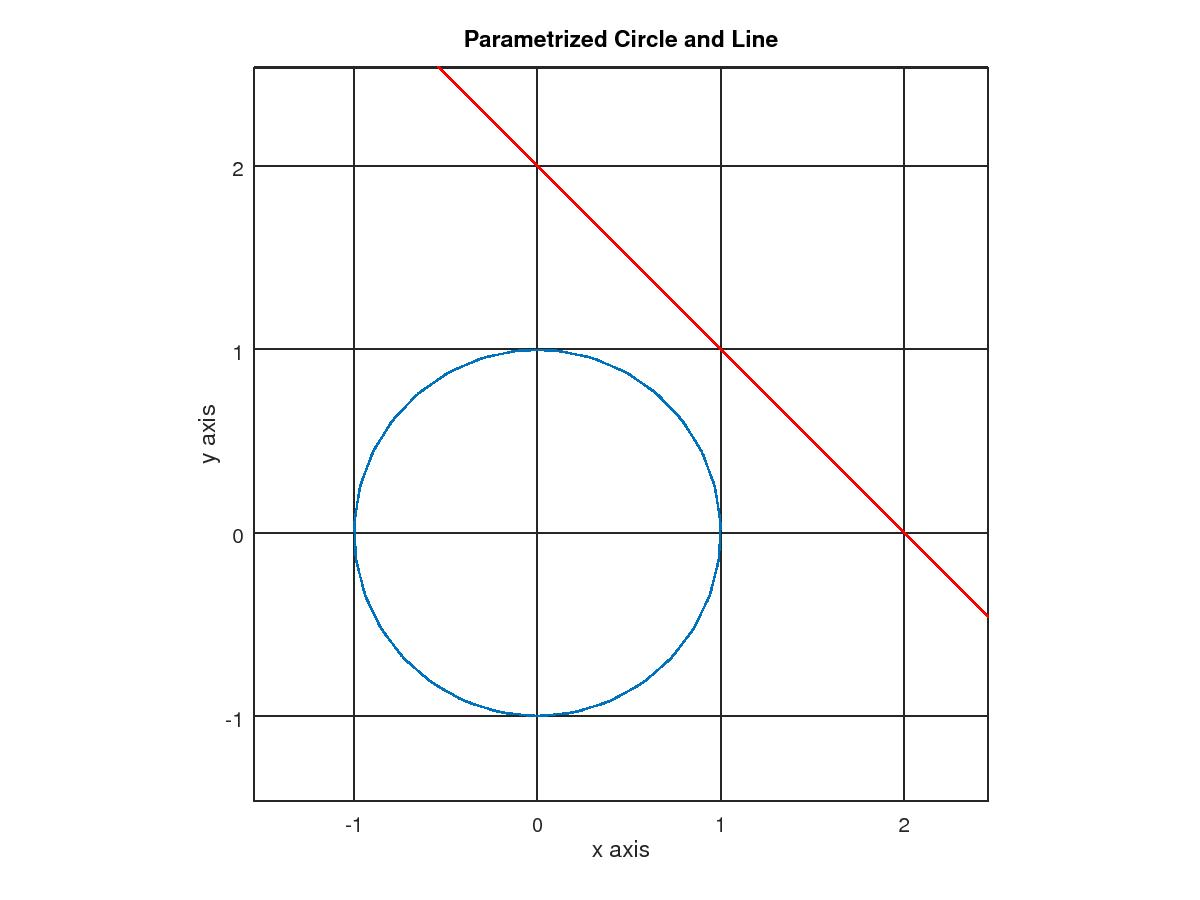
\includegraphics[scale=0.5, inner]{1}

\begin{center}
\caption{Figure 1: Parametrized unit Circle and Line}
\end{center}

\vspace{7mm}
The input functions to $razdalja$ representing the two curves can be written follows:

\begin{tcolorbox}
	\begin{small}
	\begin{verbatim}
function [r, dr, ddr] = line(s)
    r = [s; 2 - s];
    dr = [1; -1];
    ddr = [0; 0];
endfunction
	\end{verbatim}
	\end{small}
\end{tcolorbox}

\begin{tcolorbox}
	\begin{small}
	\begin{verbatim}
function [r, dr, ddr] = circle(t)
    r = [sin(t); cos(t)];
    dr = [cos(t); -sin(t)];
    ddr = [-sin(t); -cos(t)];
endfunction
	\end{verbatim}
	\end{small}
\end{tcolorbox}

Consider $t=0$ and $s=0$ to be the initial estimates for parameters $t$ and $s$.
Calling the $razdalja$ function as

\begin{tcolorbox}
	\begin{small}
	\begin{verbatim}
[d, t, s] = razdalja(@circle, @line, 0, 0)
	\end{verbatim}
	\end{small}
\end{tcolorbox}

yield the results

\begin{tcolorbox}
	\begin{small}
	\begin{verbatim}
>> t
t =  0.78540
>> s
s =  1
>> d
d =  0.41421
	\end{verbatim}
	\end{small}
\end{tcolorbox}

We can check that the vector distance vector is orthogonal to both curves at these points by computing the dot product of the distance vector with the derivatives $F'(t)$ and $G'(s)$.

\begin{tcolorbox}
	\begin{small}
	\begin{verbatim}
>> r = circle(t) - line(s)
r =

  -0.29289
  -0.29289

>> dot(r, [~, res] = circle(t))
ans =   -1.1102e-16
>> dot(r, [~, res] = line(s))
ans =   -1.1102e-16
	\end{verbatim}
	\end{small}
\end{tcolorbox}

We can see that the dot product is practically equal to zero which implies orthogonality.

The fact that the found parameters really represent the closes points can be further reaffirmed by plotting the distance vector between them.
\vspace{5mm}

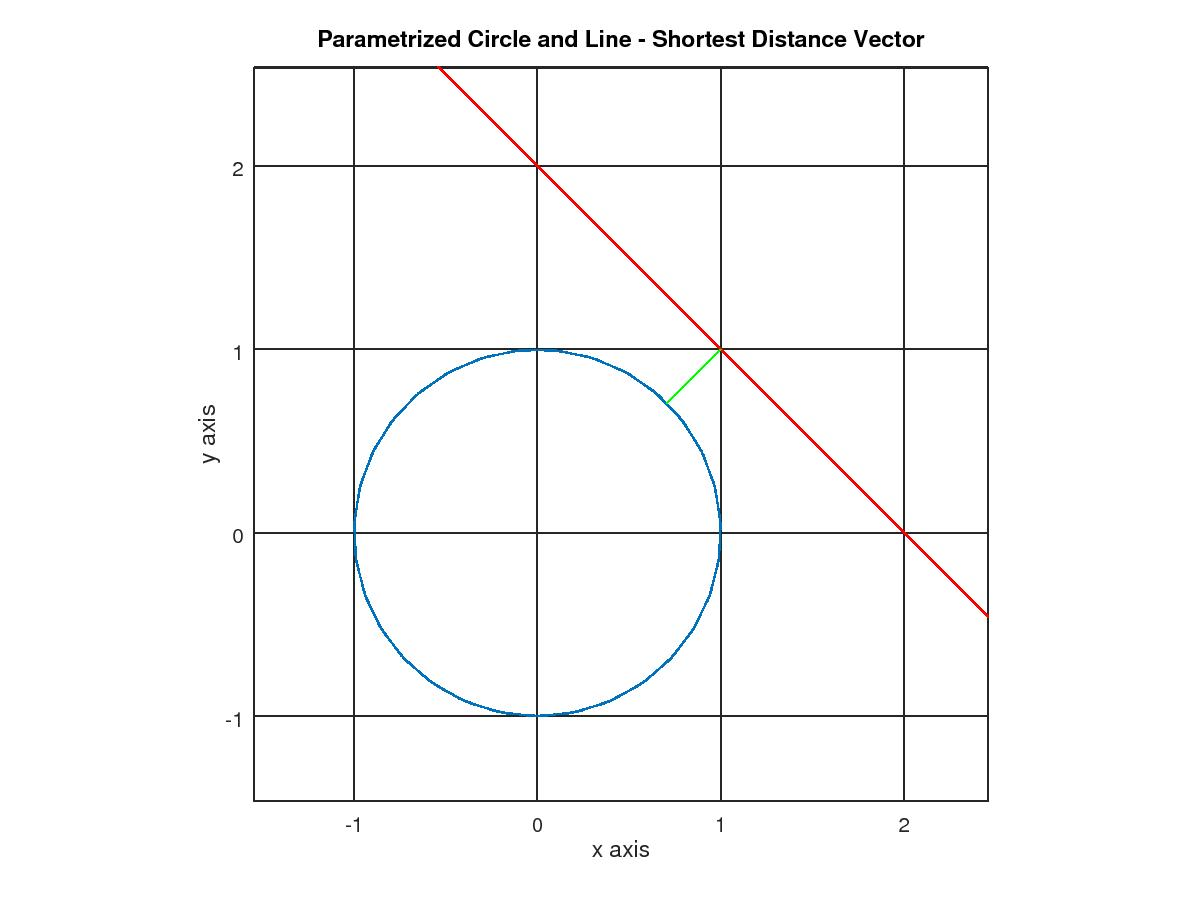
\includegraphics[scale=0.5, inner]{2}
\begin{center}
	\caption{Figure 2: Distance vector through $F(t=0.78540)$ and $G(s=1)$}
\end{center}

\end{document}